%
% File acl2021.tex
%
%% Based on the style files for EMNLP 2020, which were
%% Based on the style files for ACL 2020, which were
%% Based on the style files for ACL 2018, NAACL 2018/19, which were
%% Based on the style files for ACL-2015, with some improvements
%%  taken from the NAACL-2016 style
%% Based on the style files for ACL-2014, which were, in turn,
%% based on ACL-2013, ACL-2012, ACL-2011, ACL-2010, ACL-IJCNLP-2009,
%% EACL-2009, IJCNLP-2008...
%% Based on the style files for EACL 2006 by
%%e.agirre@ehu.es or Sergi.Balari@uab.es
%% and that of ACL 08 by Joakim Nivre and Noah Smith

\documentclass[11pt,a4paper]{article}
\usepackage[hyperref]{acl2021}
\usepackage{times}
\usepackage{latexsym}
\renewcommand{\UrlFont}{\ttfamily\small}
\usepackage{glossaries}
\usepackage[super]{nth}
\usepackage{graphicx}
\usepackage{stfloats}
\usepackage{cleveref}

\usepackage{float}
\usepackage{xcolor}
\usepackage{color, colortbl}
\usepackage{tabularx}
\newcolumntype{Z}{>{\raggedright\let\newline\\\arraybackslash\hspace{0pt}}X}
%\newcolumntype{s}{>{\raggedright\let\newline\\\arraybackslash\hspace{0pt}}0.5X}
\newcolumntype{s}{>{\hsize=0.667\hsize\arraybackslash} X}
\newcolumntype{Y}{>{\hsize=1.333\hsize\arraybackslash} X}

% This is not strictly necessary, and may be commented out,
% but it will improve the layout of the manuscript,
% and will typically save some space.
\usepackage{microtype}

\aclfinalcopy % Uncomment this line for the final submission
%\def\aclpaperid{***} %  Enter the acl Paper ID here

%\setlength\titlebox{5cm}
% You can expand the titlebox if you need extra space
% to show all the authors. Please do not make the titlebox
% smaller than 5cm (the original size); we will check this
% in the camera-ready version and ask you to change it back.

\newcommand\BibTeX{B\textsc{ib}\TeX}

\title{Swiss German Speech to Standard German Text\\
    \normalsize\textit{SwissText.org Shared Task 3}}

\author{Alex Wolf\\
  University of Zurich \\
  \texttt{alex.wolf@uzh.ch} \\\And
  Deborah Noemie Jakobi\\
  University of Zurich \\
  \texttt{deborahnoemie.jakobi@uzh.ch} \\}

\date{}
\newacronym{stcd}{STCD}{SwissText Conference dataset}
\newacronym{stc}{STC}{SwissText Conference}
\newacronym{wer}{WER}{Word Error Rate}
\newacronym{stt}{STT}{Speech-to-Text}
\begin{document}
\maketitle
\begin{abstract}
This paper presents a solution to the \gls{stc} shared task 3, 2021. The shared task challenges participants to implement models for translating Swiss German speech to standard German text. The authors implemented multiple \textit{DeepSpeech} models using the data provided by SwissText as well as additional data which lead to improvement of the model. An additional experiment with a sequence to sequence translation model was conducted in order to improve our score. We achieved a BLEU score of up to 0.17 on the test set of SwissText. Although the final model did not score well in comparison with other submissions, there is plenty of room for possible improvements.
\end{abstract}


\section{Introduction}
Automatic speech recognition (ASR) means translating a spoken utterance into written text. It can, for example, be used for voice assistants or automatic transcription of audio or video files. While pre-trained \gls{stt} models for English are available, German models or even Swiss German models are rare or not existing \cite{Agarwal2019GermanES}. Swiss German has a wide variety of different Swiss German dialects, with a huge difference in words, pronunciation, even to the point of sounding like a different language. Swiss German has relatively little speakers (around 5 million) and there is hardly any standardized spelling. This leads to Standard German being one of the official writing language in Switzerland. As there is no official Swiss German spelling, most speakers using written Swiss German just use their own spelling which resembles mostly a phonetic translation. This leads to huge variance within Swiss German writing \citep{pluss2020}. It makes therefore sense to translate spoken Swiss German to Standard German in order to correspond to the official language situation. Tackling a standardized translation of different spoken Swiss German dialects into standardized German text requires a vast amount of data and fine tuning. The \gls{stc} 2021 proposed a shared task to tackle this problem and provided a dataset
(\gls{stcd} to train and fine tune on. This paper shows what kind of experiments, data, and approaches the authors used to tackle this problem. The proposed task is very complex as it includes not only a \gls{stt} conversion but also translation from Swiss German to Standard German which can be referred to as speech translation \cite{pluss2020}. Additionally, it possibly includes domain shift, as the training data stems only from Swiss parliament speeches while the domain of the test set is unclear. 
This paper presents a overview on the previous research done within this area, an introduction to the DeepSpeech model used for tackling the task and our experiments and results.  

\section{Literature review}
The shared task of translating spoken Swiss German into standard written German was already presented by the \gls{stc} in 2020. The only difference between the tasks is that this year's task provides
more data, while last year's task was specifically about low-resource languages. While the current 2021 task is about reaching the highest BLEU score, last year's submissions were ranked based on the
least \gls{wer}. \citet{buechi2020} achieved the best \gls{wer} of 40.29\%. The authors used a CNN acoustic model named Jasper. They used additional Standard German data and fine-tuned on the official
data set. They used different augmentation techniques and a language model. \cite{Kew2020} achieved the second-best \gls{wer} of 45.45\%. They used a DNN-HMM time-delay neural model including a specifically created pronunciation lexicon.   \\
\citet{Agarwal2020LTLUDEAL} used an end-to-end model called DeepSpeech and achieved an \gls{wer} of 58.93\%. This is the model we decided to use as well. It is publicly available on GitHub and can easily be fine-tuned or used for transfer learning \citet{pluss2020}.


\section{DeepSpeech}
Mozilla DeepSpeech is an end-to-end \gls{stt} model using tensorflow. It was first developed for translating English speech to English text \cite{Hannun2014DeepSS}. \citet{Agarwal2019GermanES} have implemented a German \gls{stt} model using DeepSpeech. It is trained with machine translation techniques. They provide all of their code and pre-trained models including ready-made scripts for transfer-learning and fine-tuning (QUOTE GITHUB https://github.com/AASHISHAG/deepspeech-german). This avoids privacy issues of common web-services that require uploading potentially private data. Additionally, researchers are free to adjust and extend the model according to their requirements. DeepSpeech is a deep recurrent neural network (RNN) on character level. It can be trained using supervised learning. 

\begin{figure}[h]
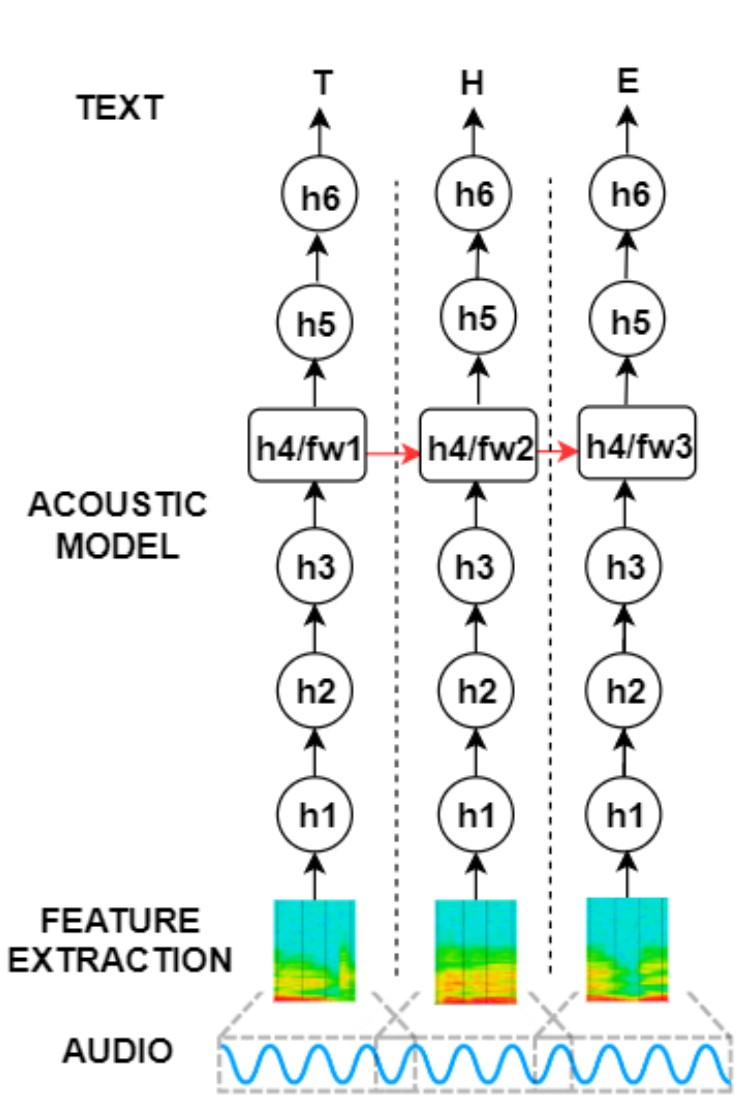
\includegraphics[scale=0.7]{deepspeech-de}
\caption{DeepSpeech architecture according to \citet{Agarwal2019GermanES}}
\label{architecture}
\end{figure}

The DeepSpeech architecture, as shown in \ref{architecture}, consists of 6 layers. A more in depth description can be found in \citet{Agarwal2019GermanES}. As becomes clear, the model has no additional phoneme-to-grapheme model but directly outputs the transcribed characters, respectively their probabilities. The Connectionist Temporal Classification (CTC) loss is used to maximize the probability of the output characters. This loss is specifically designed for tasks where the prediction categories have unclear boundaries. In this case characters which can refer to phonemes that span over times frames of various length.  
\section{Experiments}
\begin{table*}[!t]
    \centering
    \begin{tabular}{lllll}
    \hline\textbf{Model\#}    & \textbf{Data} & \textbf{Train BLEU}   & \textbf{Test BLEU}  & \textbf{WER}  \\\hline
    1                   & SwissText     & 0.23                  &  0.0004 & -              \\
    2                   & ArchiMob      & 0.27                  & \textbf{0.17}             & 0.52             \\
    3                   & ArchiMob + SwissText      & 0.28                  & 0.1                      & 0.54               \\
    4                   & ArchiMob + SwissText + text-to-text      & 0.16                  & 0.07                      & -              \\
    \hline
    \end{tabular}
    \caption{Results}
    \label{tab:Results}
\end{table*}

\subsection{Training Data}
To train our model we use a subset of the dataset provided by the \gls{stc} as well as the ArchiMob corpus. The \gls{stc} provides two different datasets. An unlabelled dataset of about 300 hours spoken Swiss German. The labeled dataset contains mostly the Bernese dialect. An additional 1200 hours of unlabeled spoken Swiss German audio data. The unlabelled dataset includes mostly the Zurich dialect. Due to time limitations, we did not use the second provided dataset. We remove all audio files from the \gls{stcd} where the quality of the translation is rated lower than 0.7 (rating provided by \gls{stc}) which are still around 130k files. Additionally, we also need to remove files larger than 1 MB due to memory limitations (ca. 7k files). All files were converted from FLAC to Wav files and the sample rate was reduced from 48'000 Hz to 16'000 Hz to match the DeepSpeech input requirements. The official test set contains 13 hours of data \cite{stc2019} and has a dialect distribution conforming to the actual Swiss German dialect distribution. In addition to the official datasets, we used the ArchiMob corpus (Release 2) which contains 57 hours of spoken Swiss German data \cite{archimob2016}. They provide Swiss German and German transcriptions and it consists of various different dialects.
The German DeepSpeech comes with a script to pre-process the transcriptions. The pre-processing includes:
\begin{itemize}
\item removing of all unallowed characters (allowed are a-zA-Zäüö)
\item convert special characters like \$ to their written form (i.e. dollar)
\item convert numbers to their written form
\item lowercase
\item map all character with diacritics to one of the allowed characters
\end{itemize}

This fits the requirements given by the \gls{stc}.

\subsection{Evaluation metrics}
We evaluate our model through two types of metrics. The BLEU score \cite{Papineni2002BleuAM}, which is required by the \gls{stc} to compare the results. The \gls{stc} specifically requires a corpus-based BLEU score, which aims at measuring the distance/similarity of the generated text and the provided ground truth. As the German DeepSpeech test script does not include the BLEU score we added it manually. \\~\\Additionally, we keep track of the \gls{wer} for our models, as
this is a common metric for speech recognition systems \cite{Park2008AnEA} which is also included in the German DeepSpeech.

\subsection{Environment}
We train the model on a single NVIDIA GeForce RTX 2070 Laptop GPU (8 GB memory). We perform minimal tuning of our model's hyperparameters following the work of \newcite{Agarwal2020LTLUDEAL}.
.

\subsection{Models}
Following \newcite{Agarwal2020LTLUDEAL} we use a DeepSpeech architecture \cite{Hannun2014DeepSS} as our main model for speech-to-text translation. In order to get better results we use a
pre-trained DeepSpeech model \cite{DeepSpeechGerman090} as the base model for most of our experiments. The first model we trained served as our private baseline. \paragraph{Baseline model} We trained a bare DeepSpeech model with the default DeepSpeech hyperparameters on the labeled \gls{stcd} which achieved a BLEU score of 0.13 on our internal test set. The baseline model will be referred to as the baseline model or model \#0 henceforth.
\paragraph{Pre-trained model \#1} In order to improve our baseline model we use a pre-trained
German DeepSpeech model \cite{DeepSpeechGerman090}, which is fine-tuned on the \gls{stcd} dataset. We used \citet{Agarwal2020LTLUDEAL} best-reported hyperparameters which are learning rate of 0.0001, dropout of 0.25. The alpha and beta values for the language model are 0.40 and 1.10 respectively. We continue to use these hyperparameters as those provided better results. The model achieved a BLEU score of
0.23 on the validation set and 0.0004 on the official test set.
\paragraph{ArchiMob data model \#2} As the \nth{1} model did not achieve the expected results we decided to fine-tune our model on the ArchiMob data, as we expected the data distribution to be closer
to the actual test set. We trained for another 30 epochs with the same hyperparameters as in model \#1. We achieved the following BLEU scores for the validation and test set, 0.27, 0.17,
respectively.
\paragraph{Augmented data model \#3} In order to produce a more robust model, that can handle different pronunciations and speeds, we added data augmentation to our \nth{2} model. We fine-tuned our
model with the following data augmentations:
\begin{itemize}
    \item warp: ''Applies a non-linear image warp to the spectrogram. This is achieved by randomly shifting a grid of equally distributed warp points along the time and frequency axis''
    \cite{DeepSpeechAugmentation}
    \item tempo: ''Scales spectrogram on the time axis and thus changes playback tempo.'' \cite{DeepSpeechAugmentation}
\end{itemize}

The \gls{stcd} dataset is used for the augmentation fine-tuning on the \nth{3} model. This approach achieved a BLEU score of 0.28 on the validation set and 0.1 on the test set. The model was trained for another
20 epochs with a warp probability of 0.1 and a tempo probability of 0.1. One epoch on this model took around 4h to complete. Due to time limitations we
were not able to continue training the model any further, but the model was still improving and we expect that this approach could produce even better results. The \gls{wer} and BLEU progression are shown in figures \ref{fig:WER} and  \ref{fig:BLEU}.
\begin{figure}[t]
    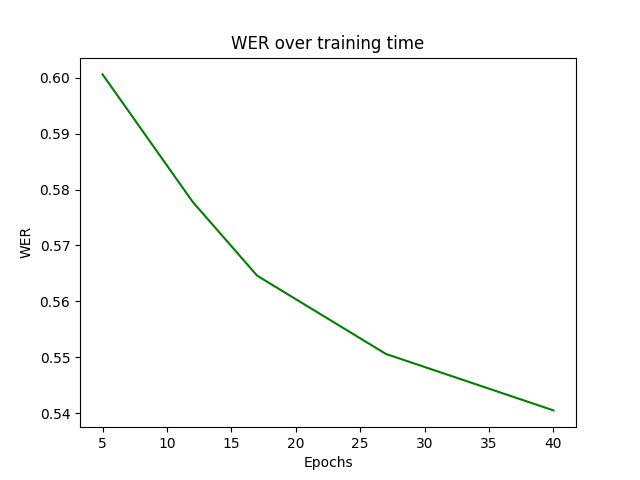
\includegraphics[width=\linewidth,height=5cm]{img/WER.png}
    \caption{WER per epoch}
    \label{fig:WER}
\end{figure}
\begin{figure}[t]
    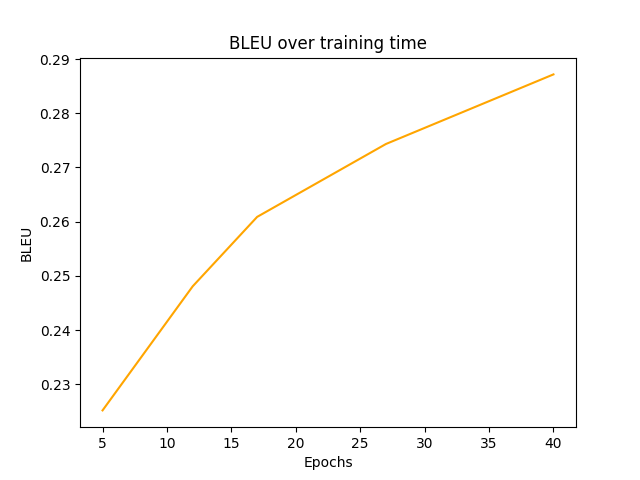
\includegraphics[width=\linewidth,height=5cm]{img/BLEU.png}
    \caption{BLEU per epoch}
    \label{fig:BLEU}
\end{figure}

\paragraph{Text-to-Text model \#4} Our \nth{4} approach tries to improve the output by adding a text-to-text translation model after the speech-to-text model. We fine-tuned a pre-trained German to
English model following \newcite{TiedemannThottingal:EAMT2020} using the ''huggingface'' framework \cite{wolf-etal-2020-transformers} on the \gls{stcd} dataset. With this approach we achieved a BLEU score of 0.13 on the validation dataset and
0.07 on the test dataset.

\section{Results \& Discussion}

Interestingly, we noticed that our internal deviations in the BLEU score are not as great as on the official test set.

\begin{table}[H]
    \centering
    \begin{tabular}{llll}
    \hline\textbf{Model\#}    & \textbf{Data} & \textbf{Train BLEU}   & \textbf{Test BLEU} \\\hline   %\\\hline %\rowcolor{gray!50}
    1                   & SwissText     & 0.23                  & 0.0004                \\%\hline %DeepSpeech (Trained from scratch)
    2                   & ArchiMob      & 0.27                  & \textbf{0.17}         \\%\hline %DeepSpeech (Pre-trained)
    3                   & ArchiMob      & 0.24                  & 0.07                  \\%\hline %DeepSpeech + Opus-MT-DE-EN (Pre-trained)
    4                   & ArchiMob      & 0.24                  & 0.07                  \\%\hline %DeepSpeech + Opus-MT-DE-EN (Pre-trained)
    5                   & ArchiMob      & 0.24                  & 0.07                  \\%\hline %DeepSpeech + Opus-MT-DE-EN (Pre-trained)
    \hline
    \end{tabular}
    \caption{\label{font-table} Font guide. }
\end{table}

%\begin{table}[b]
%    \centering
%    \begin{tabular}{lllll}
%    %\begin{tabularx}{\linewidth}{|Y|Z|Y|s|s|}
%        \hline
%        \textbf{Model#} & \textbf{Data} & \textbf{Additional information}           & \textbf{Train BLEU}   & \textbf{Test BLEU}    \\\hline %\rowcolor{gray!50}
%        1               & SwissText     & -                                         & 0.23                  & 0.0004                \\\hline %DeepSpeech (Trained from scratch)
%        2               & ArchiMob      & Fine-tuned on latest German DeepSpeech    & 0.27                  & \textbf{0.17}         \\\hline %DeepSpeech (Pre-trained)
%        3               & ArchiMob      & Additional sequence to sequence model     & 0.24                  & 0.07                  \\\hline %DeepSpeech + Opus-MT-DE-EN (Pre-trained)
%    \end{tabular}
% %   \end{tabularx}
%    \caption{Results}
%    \label{tab:Results}
%\end{table}

\section{Conclusion}


%\newpage
\bibliographystyle{acl_natbib}
\bibliography{acl2021}

%\appendix

\end{document}
